\begin{figure}[t]
  \centering
  \begin{tikzpicture}[
      node distance=1.5cm,
      block/.style={rectangle, draw, minimum width=1cm, minimum
      height=1cm, text centered},
      arrow/.style={->, >=stealth},
      label/.style={text width=2cm, align=center}
    ]

    % Input image
    \node[block] (input) {
    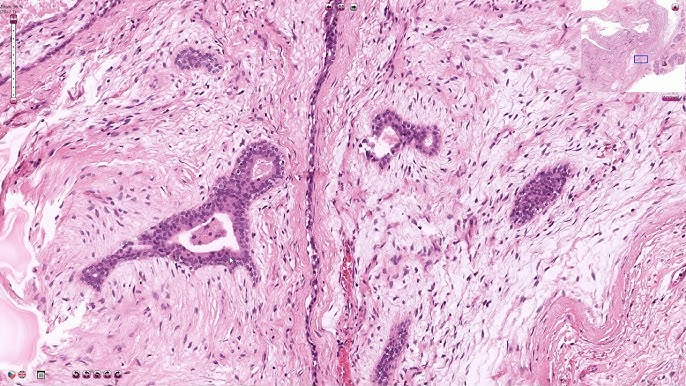
\includegraphics[width=2cm]{Cap4/Figures/histopathology_patch.jpg}};
    \node[text width=2cm, align=center, above of=input, yshift=0.5cm]
    {Input Image $\mathbf{X}$};

    % Annotator masks
    \node[block, right of=input, xshift=2cm] (mask1) {$\mathbf{Y}_1$};
    \node[block, above of=mask1] (mask2) {$\mathbf{Y}_2$};
    \node[block, below of=mask1] (mask3) {$\mathbf{Y}_R$};

    % Reliability maps
    \node[block, right of=mask1, xshift=1cm] (rel1) {$\Lambda_1$};
    \node[block, right of=mask2, xshift=1cm] (rel2) {$\Lambda_2$};
    \node[block, right of=mask3, xshift=1cm] (rel3) {$\Lambda_R$};

    % Model prediction
    \node[block, right of=rel1, xshift=2cm] (pred) {$f(\mathbf{X};\theta)$};

    % Loss computation
    \node[block, below of=pred, yshift=-2cm] (loss) {TGCE$_{SS}$ Loss};

    % Arrows
    \draw[arrow] (input) -- (mask1);
    \draw[arrow] (input) -- (mask2);
    \draw[arrow] (input) -- (mask3);

    \draw[arrow] (mask1) -- (rel1);
    \draw[arrow] (mask2) -- (rel2);
    \draw[arrow] (mask3) -- (rel3);

    \draw[arrow] (rel1) -- (loss);
    \draw[arrow] (rel2) -- (loss);
    \draw[arrow] (rel3) -- (loss);
    \draw[arrow] (pred) -- (loss);

    % Annotations
    \node[text width=2cm, align=center, above of=mask2, yshift=0.5cm]
    {Annotator Masks};
    \node[text width=2cm, align=center, above of=rel2, yshift=0.5cm]
    {Reliability Maps};
    \node[text width=2cm, align=center, above of=pred, yshift=0.5cm]
    {Model Prediction};

    % Loss components
    \node[block, below of=loss, yshift=-3cm] (reliable) {Reliable Regions Loss};
    \node[block, left of=reliable, xshift=-3cm] (unreliable)
    {Unreliable Regions Loss};

    \draw[arrow] (loss) -- (reliable);
    \draw[arrow] (loss) -- (unreliable);

    % Legend
    \node[text width=4cm, align=left, right of=loss, xshift=2cm] {
      \textbf{Loss Components:}\\
      $\bullet$ Reliable: $\Lambda_r \circ GCE$\\
      $\bullet$ Unreliable: $(1-\Lambda_r) \circ \text{Uniform Prior}$
    };

  \end{tikzpicture}
  \caption{Working mechanism of the proposed Truncated Generalized
    Cross Entropy for Semantic Segmentation (TGCE$_{SS}$) loss
    function. The loss combines reliability maps $\Lambda_r$ with the
    model's predictions $f(\mathbf{X};\theta)$ to compute a weighted
  loss that accounts for annotator reliability across different image regions.}
  \label{fig:loss_mechanism}
\end{figure}